%!TEX root = ../six_pole.tex
% Тип документа
\documentclass[a4paper,12pt]{extarticle}

% Шрифты, кодировки, символьные таблицы, переносы
% \usepackage{cmap}
% \usepackage[T2A]{fontenc}
\usepackage[utf8]{inputenc}
\usepackage[russian]{babel}
% Это пакет -- хитрый пакет, он нужен но не нужен
\usepackage[mode=buildnew]{standalone}

\usepackage
	{
		% Дополнения Американского математического общества (AMS)
		amssymb,
		amsfonts,
		amsmath,
		amsthm,
		% Пакет для физических текстов
		physics,
		% misccorr,
		% 
		% Графики и рисунки
		wrapfig,
		graphicx,
		subcaption,
		float,
		tikz,
		tikz-3dplot,
		caption,
		csvsimple,
		color,
		booktabs,
		geometry,
		% 
		% Таблицы, списки
		makecell,
		multirow,
		indentfirst,
		%
		% Интегралы и прочие обозначения
		ulem,
		esint,
		esdiff,
		% 
		% Колонтитулы
		fancyhdr,
	}  
\usepackage{pgfplots,pgfplotstable,booktabs,colortbl}
\usepackage{xcolor}
\usepackage{hyperref}

 % Цвета для гиперссылок
\definecolor{linkcolor}{HTML}{000000} % цвет ссылок
\definecolor{urlcolor}{HTML}{799B03} % цвет гиперссылок
 
\hypersetup{pdfstartview=FitH,linkcolor=linkcolor,urlcolor=urlcolor, colorlinks=true}
\hypersetup{pageanchor=false}
% Увеличенный межстрочный интервал, французские пробелы
\linespread{1.3} 
\frenchspacing 

 
% \usetikzlibrary
% 	{
% 		decorations.pathreplacing,
% 		decorations.pathmorphing,
% 		patterns,
% 		calc,
% 		scopes,
% 		arrows,
% 		fadings,
% 		through,
% 		shapes.misc,
% 		arrows.meta,
% 		3d,
% 		quotes,
% 		angles,
% 		babel
% 	}
% Среднее <#1>
\newcommand{\mean}[1]{\langle#1\rangle}
% const прямым шрифтом
\newcommand\ct[1]{\text{\rmfamily\upshape #1}}
\newcommand*{\const}{\ct{const}}
\usepackage{array}
\usepackage{pstool}

\geometry		
	{
		left			=	2cm,
		right 			=	2cm,
		top 			=	2.5cm,
		bottom 			=	2.5cm,
		bindingoffset	=	0cm
	}

%%%%%%%%%%%%%%%%%%%%%%%%%%%%%%%%%%%%%%%%%%%%%%%%%%%%%%%%%%%%%%%%%%%%%%%%%%%%%%%
	%применим колонтитул к стилю страницы
\pagestyle{fancy} 
	%очистим "шапку" страницы
% \fancyhead{} 
	%слева сверху на четных и справа на нечетных
\fancyhead[R]{}%\labauthors 
	%справа сверху на четных и слева на нечетных
% \fancyhead[L]{Отчёт по лабораторной работе №\labnumber}
\fancyhead[L]{\labtheme} 
	%очистим "подвал" страницы
% \fancyfoot{} 
	% номер страницы в нижнем колинтуле в центре
\fancyfoot[C]{\thepage} 

%%%%%%%%%%%%%%%%%%%%%%%%%%%%%%%%%%%%%%%%%%%%%%%%%%%%%%%%%%%%%%%%%%%%%%%%%%%%%%%

\renewcommand{\contentsname}{Оглавление}
\usepackage{tocloft}
\usepackage{secdot}
\sectiondot{subsection}
\usepackage{gensymb}
\usepackage{textcomp}
\usepackage{pythontex}

\begin{document}
\def\labauthors{Карусевич А.А, Понур К.А.}
\def\labgroup{430}
\def\department{Кафедра радиоэлектроники}
\def\labnumber{1}
\def\labtheme{Исследование амплитудной модуляции}

\renewcommand{\Re}{\operatorname{Re}}
\renewcommand{\Im}{\operatorname{Im}}
\renewcommand{\phi}{\varphi}
\renewcommand{\hat}{\widehat}

\begin{titlepage}

\begin{center}

{\small\textsc{Нижегородский государственный университет имени Н.\,И. Лобачевского}}
\vskip 1pt \hrule \vskip 3pt
{\small\textsc{Радиофизический факультет}}



\vfill
{\Large {\department}}

{\Large Отчет по лабораторной работе №\labnumber\vskip 12pt\bfseries \labtheme}
	
\end{center}

\vfill
	
\begin{flushright}
	{Выполнили студенты \labgroup\ группы\\ \labauthors}%\vskip 12pt Принял:\\ Менсов С.\,Н.}
\end{flushright}
	
\vfill
	
\begin{center}
	Нижний Новгород, \the\year
\end{center}

\end{titlepage}


% \tableofcontents
% \newpage


\section{Общая теория модуляции}
\subsection{Определение и классификация различных видов модуляции}

Для работы любой радиолинии необходимо, чтобы ток возбуждения антенны на её передающем конце отображал передаваемый сигнал, т.е. необходимо каким-то образом «записать» его на токе высокой частоты.

Процесс изменения параметров тока высокой частоты или параметров импульсов (при импульсной работе) в соответствии с передаваемым сигналом получил название модуляции.

При непрерывных методах передачи до осуществления модуляции ток генератора представляет собой чисто гармоническое колебание:

$$i = I_m\cos{\Phi(t)} = I_m\cos{(\omega_0 t + \varphi)},$$

где амплитуда $I_m$, частота $\omega_0$ и фаза $\varphi$ постоянны во всем интервале $(-\infty, +\infty)$ изменения времени $t$.

Полной фазой колебаний будем называть угол $\Phi(t)$, который для гармонических колебаний изменяется линейно в функции времени:

$$\Phi(t) = \omega_0 t + \varphi.$$

Можно наметить три различных пути для осуществления модуляции, т.е. можно изменять в соответствии с передаваемым сигналом амплитуду, частоту или фазу тока. Если изменять амплитуду, то модуляция называется амплитудной, при изменении фазы — фазовой, а при изменении частоты — частотной.

Следует иметь в виду, что изменение фазы всегда сопровождается изменением частоты и всякому закону изменения фазы можно найти эквивалентный закон изменения частоты. По этим соображениям иногда различают только два вида модуляции — амплитудную и фазовую (или частотную), не различая между собой фазовую и частотную модуляцию.

Однако с точки зрения радиотехнической практики все же целесообразно различать частотную и фазовую модуляцию в зависимости от того, что изменяется в соответствии с передаваемым сигналом — фаза или частота. 

При импульсной модуляции радиоимпульсы определяются амплитудой $I_m$, фазой $\varphi$ и частотой $\omega$ колебаний внутри импульсов и, кроме того, параметрами самих импульсов: их длительностью $\tau_i$, частотой $\Omega_i$ и фазой следования $\varphi_i$.

Частота и фаза следования импульсов ($\Omega_i$ и $\varphi_i$), так же как частота и фаза высокочастотных колебаний ($\omega$ и $\varphi$), связаны между собой ($\Omega_i=\frac{d\varphi_i}{dt}$).

При импульсных методах передачи полоса частот, занимаемая сигналом, в основном определяется длительностью импульсов. При кратковременных импульсах, порядка микросекунд, полоса частот имеет значительную величину, порядка нескольких мегагерц. С такой широкой полосой частот можно передавать сигналы только в диапазоне ультракоротких волн. Наибольшее распространение в этом диапазоне получили фазовая и частотная импульсные модуляции (ФИМ и ЧИМ).

Различные виды модуляции при импульсной и непрерывной работе можно также классифицировать, исходя из их назначения. 

Модуляция, осуществляемая для передачи телеграфных сигналов, называется телеграфной модуляцией или манипуляцией. Модуляция же, осуществляемая для передачи речи, называется телефонной модуляцией. Если модуляция предназначена для передачи телевизионных сигналов, то она может быть названа телевизионной модуляцией или видео модуляцией.

Модуляция в радиолиниях, имеющих несколько каналов, т.е. предназначенных для одновременной передачи нескольких различных сигналов, называется многоканальной модуляцией. 

\subsection{Основные показатели, характеризующие модуляцию}

При сравнении различных методов модуляции наиболее важным показателем является помехоустойчивость, которая в значительной степени определяет надежность и дальность радиосвязи.

Детальное изучение различных видов модуляции показывает, что для передачи какого-либо сигнала $I(t)$ требуется вполне определенная полоса частот. При различных способах модуляции эта полоса частот при передаче одного и того же сигнала различна. В некоторых случаях, например при амплитудной модуляции, полоса частот, занимаемая модулированными высокочастотными колебаниями, только в два раза шире полосы частот сигнала $I(t)$. Такие методы модуляции получили название узкополосных. В других
случаях полоса частот модулированных колебаний значительно превосходит
полосу частот сигнала $I(t)$. Такие методы модуляции получили название
широкополосных. 

Следует иметь в виду, что полоса частот, занимаемая той или иной радиолинией, далеко не всегда определяется только полосой частот, необходимой для передачи радиосигнала. Указанная полоса частот в ряде случаев, особенно в области ультракоротких волн, определяется нестабильностью частоты передатчика или приемника радиолинии. При выборе
того или иного метода модуляции существенно правильно согласовать полосу частот, занимаемую передаваемым радиосигналом, с полосой частот радиолинии, определяемой нестабильностью ее несущей частоты.

Таким образом, полоса частот, требующаяся для передачи одного и того же сигнала и различная при различных методах модуляции, также является одним из важных показателей метода модуляции.

Далее, от метода модуляции и от способа осуществления модуляции зависит к.п.д. генератора, а также использование генераторной лампы по мощности. В связи с этим дальность радиосвязи при заданной номинальной мощности передатчиков, но при различных методах осуществления модуляции, может оказаться различной.

Наконец, важным показателем качества модуляции является точность воспроизведения передаваемого сигнала в радиоприемном устройстве. 

Заметим, что качество воспроизведения в большей степени зависит от способа осуществления модуляции, чем от метода модуляции.

Таким образом, при оценке различных методов модуляции, а также различных способов осуществления модуляции, необходимо исходить из следующих основных показателей: помехоустойчивости, т. е. степени влияния помех на передаваемый сигнал; спектра частот, необходимого для передачи сигнала; к.п.д. модулируемого генератора; использования по мощности активных элементов модулируемого генератора; дальности действия радиостанции при заданной номинальной мощности передатчика; простоты
осуществления; габаритов и веса передатчика и приемника.

\section{Амплитудная модуляция}
\subsection{Математическое выражение модулированных колебаний}

Допустим, что передаваемый сигнал $I(t)$ представляет собой гармоническое колебание звуковой частоты $\Omega$ (рис.1а). При амплитудной модуляции амплитуда тока высокой частоты должна изменяться в соответствии с этим сигналом. Такое модулированное колебание показано на рис.1б.

\begin{figure}[h!]
	\centering
	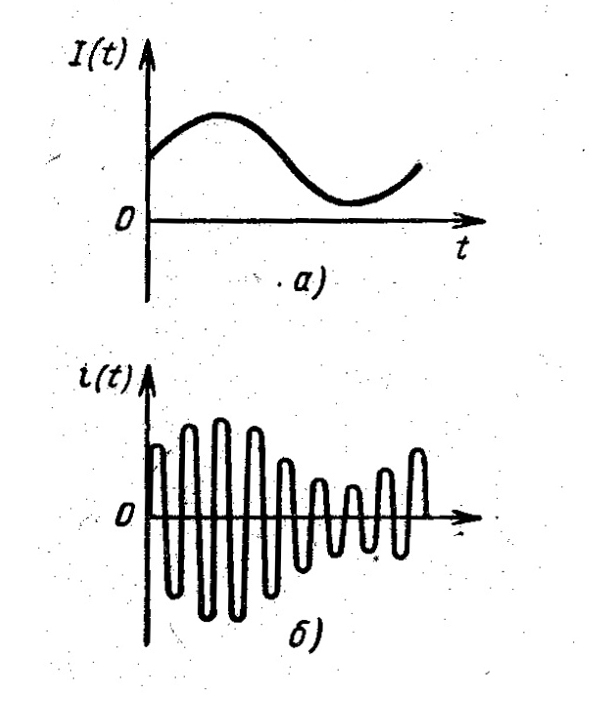
\includegraphics[width=0.5\linewidth]{fig/fig1}
	\caption{Амплитудная модуляция (а - сигнал; б - модулированное колебание, соответствующее сигналу).}
	\label{fig:fig1}
\end{figure}

Если обозначить через $I_{\text{н}}$ амплитуду высокочастотного колебания до
осуществления модуляции и предположить, что во время модуляции изменение амплитуды $I_m$ прямо пропорционально силе звука нашего сигнала, то закон изменения амплитуды тока высокой частоты при модуляции чистым тоном
звуковой частоты $\Omega$ запишется так: 

$$I_{\text{н}}+I_1\cos{\Omega t},$$

\begin{equation}
	i = I_{\text{н}}(1+m\cos{\Omega t})\cos{\omega_0 t},
\end{equation}
где $m=\frac{I_1}{I_{\text{н}}}$ - коэффициент модуляции.

\subsection{Анализ модулированных колебаний}

После несложных преобразований выражение (1) может быть представлено следующим образом: 

\begin{equation}
	i = I_{\text{н}}\cos{\omega_0 t}+mI_{\text{н}}\cos{\Omega t}\cos{\omega_0 t}
\end{equation}
или
\begin{equation}
	i = I_{\text{н}}\cos{\omega_0 t}+\frac12mI_{\text{н}}\cos{(\omega_0+\Omega)t}+\frac12mI_{\text{н}}\cos{(\omega_0-\Omega)t}.
\end{equation}

Из полученного выражения видно, что колебание, модулированное одной звуковой частотой $\Omega$ ($\Omega$— частота модуляции), состоит из трех гармонических колебаний.

Первое колебание частоты $\omega_0$ имеет амплитуду, равную амплитуде колебания до осуществления модуляции; второе и третье колебания частот $\omega_0+\Omega$ и $\omega_0-\Omega$ имеют амплитуды, равные $\frac12mI_{\text{н}}$, т.е. их амплитуды прямо пропорциональны коэффициенту модуляции. Частота $\omega_0$ называется несущей частотой, частоты $\omega_0+\Omega$ и $\omega_0-\Omega$ боковыми частотами.

Спектр модулированных колебаний можно наглядно представить в виде графика, откладывая по горизонтальной оси частоты, а по вертикальной – амплитуды тех колебаний, которые входят в состав модулированного тока. Колебание, модулированное одной звуковой частотой $\Omega$, будет иметь спектр, состоящий из несущей и двух боковых частот (Рис.2а).

\begin{figure}[h!]
	\centering
	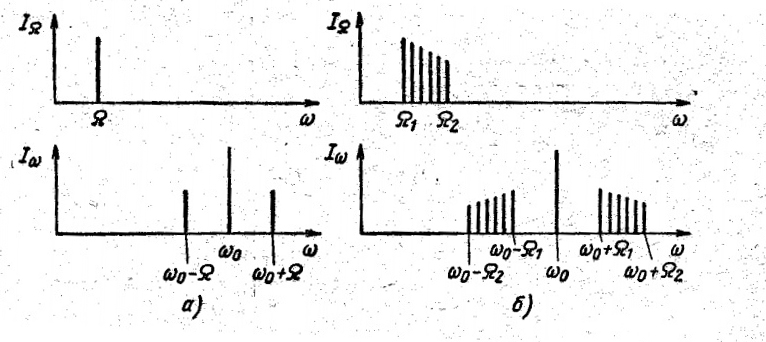
\includegraphics[scale=1.5]{fig/fig2}
	\caption{ Частотные спектры сигналов и колебаний высокой частоты,
	модулированных по амплитуде в соответствии с этими сигналами.}
	\label{fig:fig2}
\end{figure}

Если звуковой сигнал содержит в себе непрерывную полосу частот от $\Omega_1$ до $\Omega_2$, то спектр модулированного колебания будет состоять из несущей частоты и двух боковых полос частот (Рис.2б).

\section{Однополосная модуляция}
\subsection{Принцип действия и основные особенности}

Для передачи информации на дальние и сверхдальние расстояния в настоящее время широко применяются системы связи с одной боковой полосой, обеспечивающие при одинаковой мощности передатчика значительно более высокую надежность связи по сравнению с системами, в которых используется обычная амплитудная модуляция.

Прежде чем перечислить основные преимущества и недостатки систем с одной боковой полосой, кратко остановимся на принципе их работы, в частности на простейшем способе образования однополосного сигнала и его отличии от обычного сигнала с амплитудной модуляцией.

\begin{figure}[H]
	\centering
	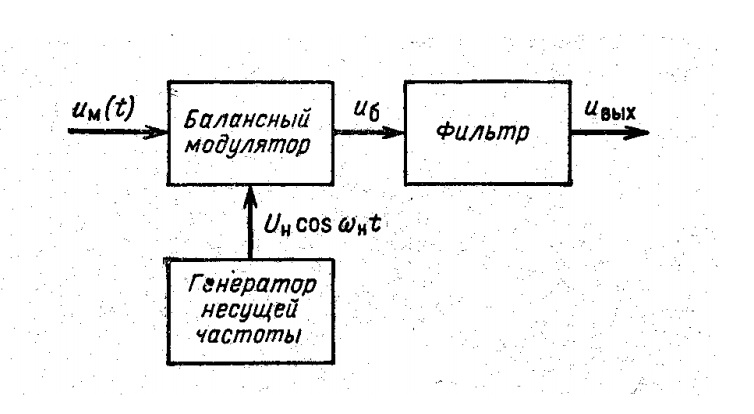
\includegraphics[width=0.5\linewidth]{fig/fig3}
	\caption{ Блок-схема формирования однополосного сигнала.}
	\label{fig:fig3}
\end{figure}

Для образования однополосного сигнала, т. е. сигнала, содержащего только верхнюю или нижнюю боковую полосу, используются балансные модуляторы. Ко входу такого модулятора (Рис.3.) одновременно подводятся напряжение передаваемого сигнала (спектр которого показан на (Рис.4а) и напряжение несущей частоты. На выходе модулятора сохраняются только
верхняя и нижняя боковые полосы (Рис.4б). 

Для получения однополосного сигнала с помощью фильтра вырезается верхняя или нижняя боковая полоса (Рис.4в), которая после усиления в высокочастотном тракте передатчика поступает в антенну и излучается.

Нетрудно видеть, что спектр однополосного сигнала по форме совпадает со спектром исходного модулирующего напряжения, однако он смещен на частоту $\omega_0$ в область более высоких частот. Информация, содержащаяся в одной боковой полосе, является недостаточной для восстановления передаваемого сигнала. Дело в том, что если нам неизвестно значение несущей частоты, то мы не сможем определить частоты передаваемого сигнала.

\begin{figure}[h!]
	\centering
	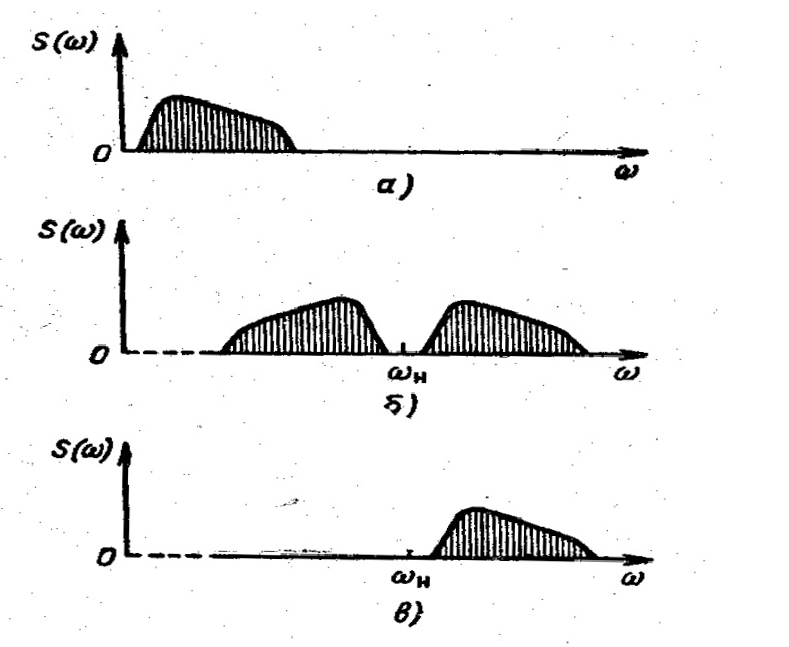
\includegraphics[scale=1.5]{fig/fig4}
	\caption{ Графики спектральной плотности сигналов: а) модулирующего;
б) двухполосного (без несущей); в) однополосного.}
	\label{fig:fig4}
\end{figure}

Таким образом, при приеме однополосного сигнала необходимо в точке приема восстанавливать несущую частоту. Остановимся на некоторых особенностях систем однополосной передачи.

К числу основных преимуществ таких систем по сравнению с обычными
амплитудно-модулированными системами можно отнести:
\begin{itemize}
	\item устранение из спектра несущей частоты и одной боковой полосы, для
передачи которых в обычных системах затрачивается значительная мощность;
	\item уменьшение полосы частот, занимаемой передатчиком, дающее возможность увеличить число станций, работающих без взаимных помех в заданном диапазоне, и существенно снизить искажение передаваемого сигнала, вызванное селективным «замиранием», которое является следствием неодинаковости условий распространения различных по частоте составляющих
спектра сигнала;
	\item сужение полосы пропускания приемного устройства, позволяющее примерно в два раза снизить мощность помех на входе приемника. 
\end{itemize}

Говоря об энергетических преимуществах рассматриваемых систем, следует заметить, что при отсутствии модулирующего сигнала (например, при молчании перед микрофоном) передатчик не излучает, в то время как в обычных системах излучается несущая частота. Учитывая, что подобные паузы при радиотелефонной передаче составляют значительную часть времени работы, применение однополосной передачи дает дополнительный, существенный энергетический выигрыш.

Полный энергетический выигрыш по сравнению с системой обычной амплитудной модуляции приблизительно оценивается в 15 — 20 раз. 

К основным недостаткам систем однополосной передачи следует отнести:
\begin{itemize}
	\item Необходимость обеспечения высокой стабильности частоты передатчика и генератора несущей частоты, восстанавливаемой на приемном конце. Отклонение восстановленной в приемнике несущей частоты от подавленной в передатчике при коммерческой связи обычно не превышает 50 — 100 Гц. Если разница превосходит указанное значение, то резко снижается
разборчивость передаваемой речи. Хорошая разборчивость речи получается, если отклонение не превышает 15 — 20 Гц. Для высококачественного приема музыкальных передач допустимая величина отклонения измеряется единицами и даже долями герца.
	\item Усложнение приемной и передающей аппаратуры, связанное с формированием однополосного сигнала, а также с восстановлением несущей частоты при демодуляции в приемном устройстве. 
\end{itemize}
Так как к точности восстановленной несущей частоты и строгости ее поддержания постоянной предъявляются высокие требования, то для контроля или автоматической подстройки несущей частоты вместе с однополосным сигналом может передаваться или значительно ослабленная несущая частота или так называемый пилот-сигнал. В ряде случаев оказывается нецелесообразным сохранять несущую частоту во всем тракте формирования однополосного сигнала, а удобнее «замешивать» ее в передаваемый сигнал в выходных каскадах передатчика.

Необходимость достаточно точного восстановления несущей частоты затрудняет использование однополосной связи с быстро летящими объектами, так как при изменении направления движения и скорости объекта вследствие влияния эффекта Доплера наблюдается заметное отклонение частоты принимаемых сигналов от частоты сигналов, излучаемых передатчиком.

При осуществлении однополосной связи с быстролетящими объектами необходимо компенсировать доплеровский сдвиг частоты. Это можно сделать, например, используя автоматическую подстройку частоты по пилот-сигналу.

Для повышения коэффициента полезного действия передатчиков с одной боковой полосой целесообразно формирование однополосного сигнала производить в маломощных каскадах передатчика, а затем усиливать его до необходимого уровня в последующих каскадах передатчика. При этом следует иметь в виду, что при выделении одной боковой полосы из амплитудно-модулированного колебания на выходе фильтра получается колебание с
амплитудно-частотной модуляцией.

Из этого свойства однополосного сигнала следует первая особенность усилительного тракта рассматриваемых передатчиков, а именно недопустимость использования в усилительном тракте каскадов умножения частоты.

Второй важной особенностью усилительного тракта однополосного передатчика являются высокие требования к линейности его амплитудной характеристики. Допустимый уровень нелинейных искажений значительно ниже, чем в обычных передатчиках. Это объясняется тем, что если среднее значение огибающей амплитудно-модулированного сигнала не зависит от характера модулирующего сигнала и определяется амплитудой колебания несущей частоты, то среднее значение огибающей однополосного сигнала зависит от величины модулирующего напряжения и обычно заметно ниже среднего значения амплитудно-модулированного сигнала. Очевидно, что в результате снижения среднего уровня сигнала усиление происходит на нижнем
участке амплитудной характеристики каскадов передатчика, и поэтому для предотвращения сильных искажений необходимо обеспечивать высокую линейность не только основной части амплитудной характеристики усилителя, но и ее начального участка. Так как усилительные каскады передатчика обычно работают с отсечкой анодного тока, т. е. в режиме колебаний 2-го рода, получение высокой линейности начального участка амплитудной характеристики усилителя обычно сопряжено с определенными трудностями и в ряде случаев требует применения специальных, активных элементов, имеющих линейный нижний участок статической характеристики выходного тока. 

Для формирования однополосного сигнала в настоящее время
используются три основных метода: 
\begin{itemize}
	\item фильтровой;
	\item фазокомпенсационный;
	\item фазофильтровой.
\end{itemize} 

\subsection{Фильтровой метод}

При высокой несущей частоте в ряде случаев возникают определенные технические трудности выделения только одной боковой полосы.

Действительно, если, например, нижняя граница спектра передаваемого звукового сигнала равна 200 Гц, то нижняя и верхняя боковые полосы будут удалены друг от друга на 400 Гц. При несущей частоте 10 МГц это составит 0,004\%. Разделение столь близко расположенных полос с помощью даже весьма совершенных кварцевых фильтров в этом диапазоне частот чрезвычайно сложно. Чтобы обойти указанное затруднение, обычно используют промежуточное преобразование частоты. 

\begin{figure}[h!]
	\centering
	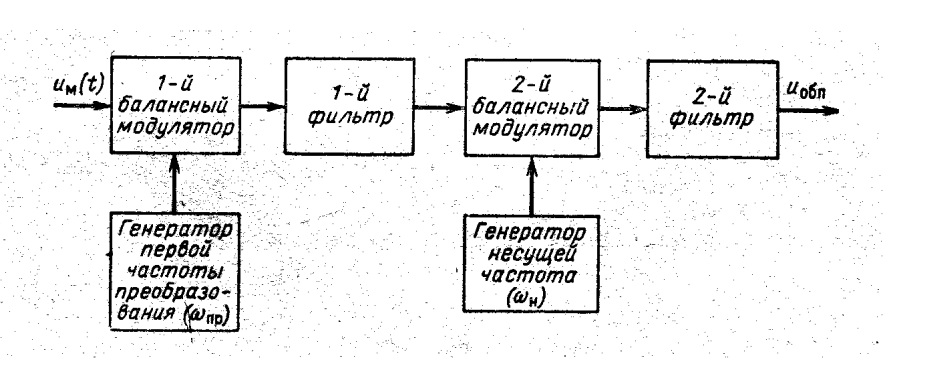
\includegraphics[width=0.8\linewidth]{fig/fig5}
	\caption{ Блок-схема формирования однополосного сигнала фильтровым методом.}
	\label{fig:fig5}
\end{figure}

В качестве примера на Рис.5 приведена блок-схема, а на Рис.6 - спектры сигнала на выходе отдельных элементов схемы, поясняющие формирование однополосного сигнала с одним
промежуточным преобразованием частоты.

\begin{figure}[h!]
	\centering
	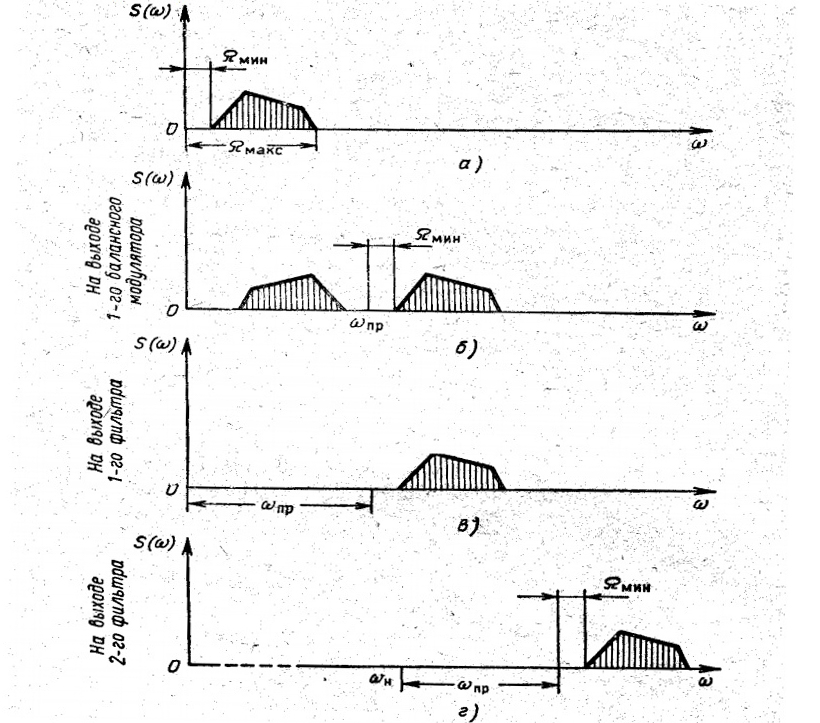
\includegraphics[scale=1.5]{fig/fig6}
	\caption{. Спектры сигнала, поясняющие формирование однополосного сигнала
фильтровым методом: а) исходного; б) на выходе первого модулятора; в) на
выходе первого фильтра; г) на выходе второго фильтра.}
	\label{fig:fig6}
\end{figure}

В данном случае предварительно получается однополосный сигнал на более низкой частоте ($\omega_{\text{пр}}$) по сравнению с несущей, что облегчает фильтрацию одной боковой полосы. Полученный на выходе фильтра сигнал (Рис. 6в), занимающий полосу частот, равную полосе частот входного сигнала, но смещенный по частоте на величину первой промежуточной частоты преобразования $\omega_{\text{пр}}$ (которую иногда называют поднесущей), подается на второй балансный модулятор, на выходе которого получаются две боковые
полосы частот, разнесенные на величину 2($\omega_{\text{пр}}+\Omega_{\text{мин}}$). С выхода балансного модулятора сигнал поступает на второй фильтр для выделения одной боковой полосы.

В данном примере использовано одно промежуточное преобразование. В ряде случаев для получения необходимого подавления несущей и нежелательной боковой полосы приходится использовать несколько подобных преобразований. По этой причине рассмотренный метод получения однополосного сигнала называется в литературе также методом
последовательных преобразований. 

\subsection{Сравнение методов формирования однополосного сигнала}

Различные методы формирования однополосного сигнала имеют свои преимущества и недостатки.

Одним из основных достоинств фазокомпенсационного метода формирования однополосного сигнала по сравнению с фильтровым методом является то, что при его использовании отпадает необходимость применения фильтров с крутым спадом характеристики в области граничных частот. Это, в свою очередь, позволяет использовать в балансных модуляторах непосредственно несущую частоту без многократного частотного преобразования, к которому мы прибегаем в случае подавления одной боковой полосы с помощью фильтров.

Недостатком фазокомпенсационного метода является необходимость использования фазовращателей, обеспечивающих постоянный фазовый сдвиг в широком диапазоне модулирующих частот, а также точный баланс схемы. К недостаткам этого метода относится также применение двух балансных
модуляторов. Указанный недостаток устраняется в многофазных системах, которые позволяют осуществить подавление несущей частоты без балансных модуляторов.

Основным преимуществом фазофильтрового метода перед фильтровым и фазокомпенсационным является отсутствие сложных фазосдвигающих схем, работающих в некотором диапазоне частот, и фильтров с крутыми спадами частотной характеристики. К фильтрам нижних частот, используемым в фазофильтровых схемах, не предъявляются требования резкого спада характеристики в области граничной частоты. 

\section{Балансные модуляторы}

Схема простейшего балансного модулятора приведена на Рис.7. Модулятор состоит из трансформатора $\text{Тр}_1$ на вход которого подается модулирующее напряжение $U_m(t)$ (например, звуковое напряжение в радиотелефонных передатчиках), двух полупроводниковых диодов $\text{Д}_1$ и $\text{Д}_1$, контура LС с катушкой связи $L_{\text{св}}$ с которой снимается выходное напряжение, и высокочастотного трансформатора $\text{Тр}_2$, обеспечивающего подачу напряжения несущей частоты. Конденсаторы $C_0$ шунтируют обмотки трансформатора $\text{Тр}_2$, по несущей частоте. Их сопротивление для модулирующего напряжения должно быть велико. 

\begin{figure}[h!]
	\centering
	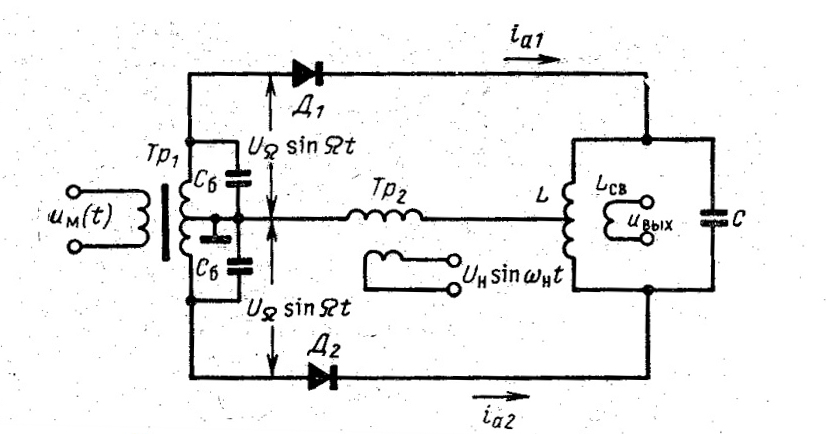
\includegraphics[width=0.8\linewidth]{fig/fig7}
	\caption{Схема балансного модулятора.}
	\label{fig:fig7}
\end{figure}

Предположим, что нелинейные элементы $\text{Д}_1$ и $\text{Д}_1$ имеют одинаковые
характеристики

$$i_a = a_1 + a_2u + a_3u^2+...,$$ 
%не 3 ли
где $u$ — действующее на элементах напряжение. 

Как видно из рис.7 напряжение несущей частоты $u_{\text{н}} = U_{\text{н}}\sin{\omega_{\text{н}}t}$ на оба диода подается в фазе, а модулирующее напряжение, снимаемое со вторичной обмотки трансформатора $\text{Тр}_1$ — в противофазе. В рассматриваемом случае,
когда модулирующее напряжение имеет синусоидальный характер, получим для напряжений на первом и втором диодах следующие выражения:

$$u_1 = U_{\Omega} \sin{\Omega t}+U_{\text{н}}\sin{\omega_{\text{н}}t},$$
$$u_2 = -U_{\Omega} \sin{\Omega t}+U_{\text{н}}\sin{\omega_{\text{н}}t}.$$

Подставляя $u_1$ и $u_2$ в выражение для тока $i_a$, ограничиваясь тремя первыми членами и учитывая, что диоды включены навстречу друг другу, получим для тока, протекающего через контур, следующее выражение: 

\begin{gather*}
	i_{\text{н}} = i_{a1} - i_{a2} = 2a_1U_2 \sin{\Omega t} + 2U_{\text{н}} U_{\Omega}\sin{\Omega t} \sin{\omega_{\text{н}}t} = \\
	2a_1U_{\Omega} \sin{\Omega t} + U_{\text{н}} U_{\Omega}[\cos{(\omega_{\text{н}}-\Omega)t}-\cos{(\omega_{\text{н}}+\Omega)t}].
\end{gather*}
Из последнего выражения видно, что на выходной обмотке $L_{\text{св}}$, симметрично связанной с катушкой контура $L$, будут выделяться только верхняя и нижняя боковые частоты: $\omega_{\text{н}}-\Omega$ и $\omega_{\text{н}}+\Omega$.

Очевидно, что для эффективной работы балансного модулятора (хорошего подавления несущей частоты) необходимо обеспечить полную симметрию схемы, идентичность нелинейных элементов, а в случае небольшого разброса их параметров — тщательную балансировку схемы,
например, с помощью дополнительных сопротивлений, включенных последовательно с нелинейными элементами.

Однако даже при полной симметрии схемы в рассмотренном виде, балансного модулятора уровень нежелательных гармоник в ряде случаев оказывается весьма высоким. Нетрудно показать, что если учесть в характеристике нелинейных элементов дополнительные члены третьей и более высоких степеней, то в выражении для выходного напряжения появляются нечетные гармоники частоты $\Omega$ и боковые частоты, обусловленные нечетными гармониками $\Omega$ и гармониками $\omega_{\text{н}}$. Для снижения уровня гармоник широко используется так называемая кольцевая схема балансного модулятора, содержащая четыре нелинейных элемента (Рис.8а). Кольцевой модулятор, по существу, представляет собой два включенных на общую нагрузку балансных модулятора, обеспечивающих двухтактный режим работы. 

\begin{figure}[h!]
	\centering
	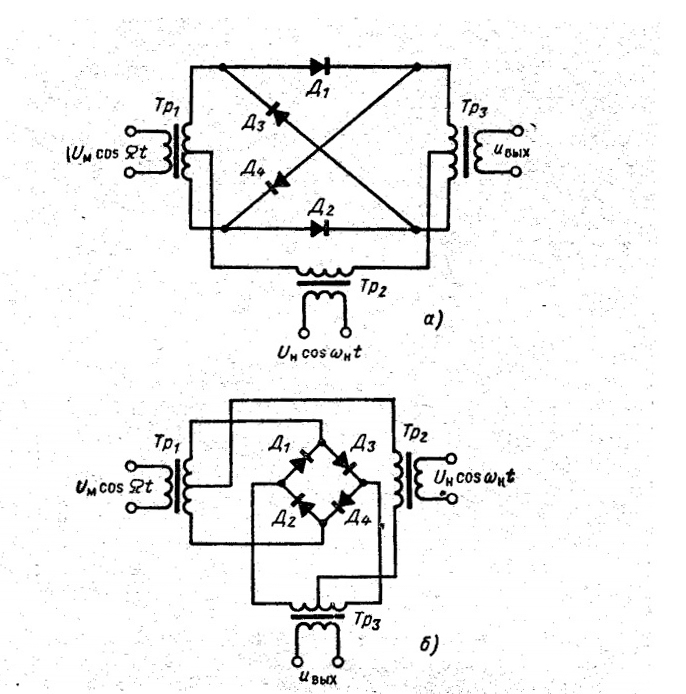
\includegraphics[width=0.8\linewidth]{fig/fig8}
	\caption{ Схема кольцевого модулятора: а) в обычном начертании: б) в виде
мостовой схемы.}
	\label{fig:fig8}
\end{figure}

Если изобразить схему Рис.8а в несколько ином виде (Рис.8б), то хорошо видно, что она представляет собой мостовую схему. При симметрии этой мостовой схемы на выходе балансного модулятора будет отсутствовать несущая частота $\omega_{\text{н}}$.

В кольцевом балансном модуляторе подавляются все нечетные гармоники$\text{Тр}_1$ частоты $\Omega$ и все боковые, образованные четными гармониками несущей частоты $\omega_{\text{н}}$.

При конструировании балансных кольцевых модуляторов, как уже отмечалось, особое внимание необходимо обращать на обеспечение симметрии схемы, которая зависит от правильного подбора нелинейных элементов (диодов), от выполнения трансформаторов (в частности, выводов средней точки) и конструкции модулятора в целом.

При высокой несущей частоте на симметрию схемы балансного модулятора могут оказывать сильное влияние паразитные параметры схемы: распределенные емкости, индуктивности и не предусмотренные расчетом связи между отдельными элементами схемы.

В кольцевой схеме балансного модулятора обычно достигается подавление несущей частоты порядка 20 — 30 дБ.

При формировании однополосного сигнала с помощью рассмотренного ранее фильтрового метода часто используется сравнительно низкая несущая частота (или частота преобразования), порядка 10 — 50 кГц. В этом случае элементы балансного модулятора $\text{Тр}_2$ и $\text{Тр}_1$ в отличие от элементов модулятора, представленного на рис.7, выполняются на ферритах или на сердечниках из трансформаторного железа. На рис.8,а показана схема кольцевого модулятора, в котором используется сравнительно низкая несущая частота $\omega_{\text{н}}$ и поэтому трансформаторы выполнены с железным сердечником.

\section{Полосовые фильтры}

В рассмотренных выше способах формирования однополосного сигнала широко используются полосовые фильтры, которые обеспечивают выделение колебаний определенных частот и подавление колебаний вне полосы пропускания фильтра. В зависимости от способа формирования, а также требований к системе связи в целом к фильтрам предъявляются различные электрические и конструктивные требования.

К основным электрическим показателям фильтров для систем формирования однополосного сигнала относятся полоса пропускания, полоса фильтрации, полоса подавления и величины затухания в каждой из полос. Все эти электрические свойства обычно представляются в виде частотной зависимости коэффициента передачи или затухания. На рис.9 приведена частотная характеристика фильтра, т.е. зависимость затухания фильтра от частоты, и обозначены характерные области частотной характеристики. 

\begin{figure}[h!]
	\centering
	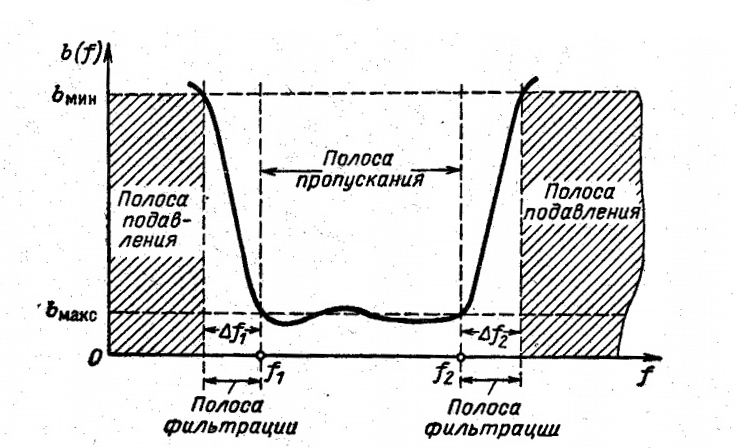
\includegraphics[width=0.8\linewidth]{fig/fig9}
	\caption{ Частотная характеристика фильтра.}
	\label{fig:fig9}
\end{figure}

Полоса пропускания ($f_2 - f_1$ на рис.9) должна соответствовать ширине спектра полезного сигнала. Затухание в полосе от $f_1$ до $f_2$ обычно составляет не более единиц децибел. Изменение затухания в полосе пропускания, определяющее амплитудные искажения пропускаемого спектра, не должно превышать долей децибела.

Фильтр должен иметь достаточно крутой спад частотной характеристики в полосах фильтрации, так как от крутизны этого спада зависят избирательные свойства фильтра. Крутизна спада частотной характеристики в полосе фильтрации обычно характеризуется производной $K_f = \frac{db}{df}$ или приближенно величиной $K_f = \frac{b_{min} - b_{max}}{\Delta d}$ (рис.9).

В полосе подавления фильтр должен иметь большое затухание, порядка 50 — 60 дБ. При недостаточном затухании возможно проникновение помех из соседних каналов. 

Кроме удовлетворения отмеченных выше, требований, фильтр должен обладать достаточной стабильностью параметров, механической прочностью, малым весом.

В реальной аппаратуре используются фильтры типа $LC$, т. е. фильтры, состоящие из элементов с сосредоточенными параметрами (катушек и конденсаторов), пьезоэлектрические и электромеханические.

Фильтры типа $LC$ имеют хорошие электрические характеристики, достаточно просты в изготовлении и находят широкое применение в схемах формирования однополосного сигнала. На частоте порядка 40 — 50 кГц они позволяют обеспечить крутизну спада частотной характеристики $K_f = 0.1 - 0.2$ дб/Гц и относительную полосу пропускания (отношение полосы пропускания $f_2 — f_1$ к средней частоте фильтра $f_0 = \frac{f_2 - f_1}{2}$) порядка $(5 - 10) 10^{-2}$.

Пьезоэлектрические фильтры, в которых используются резонаторы из кварца, турмалина, титаната бария и других материалов, обладающих пьезоэлектрическим эффектом, позволяют обеспечить более высокие избирательные свойства по сравнению с фильтром $LC$. Из упомянутых материалов, в которых проявляется пьезоэффект, в фильтрах систем
однополосной передачи применяется главным образом кварц. Резонаторы из кварца обладают высокой добротностью и хорошими эталонными свойствами, т. е. высокой стабильностью электрических параметров. Применение кварцевых резонаторов в фильтрах обеспечивает получение более высокой крутизны спада частотной характеристики фильтра и относительной полосы пропускания порядка $5 \ast 10^{-4}$.

К недостаткам кварцевых фильтров следует отнести сложность изготовления (в частности, подгонки частоты) кварцевых резонаторов, а также сложность настройки фильтров и их высокую стоимость.

В электромеханических фильтрах используются механические колебания резонаторов, изготовленных из металлических сплавов, обладающих высокой стабильностью (например, инвара, сплава никеля с железом и т. п.). 

Электромеханический фильтр представляет собой набор резонаторов цилиндрической, прямоугольной или другой формы (до 10 — 15 штук), соединенных металлическими связками, форма которых может быть также различной (рис. 10).  

\begin{figure}[h!]
	\centering
	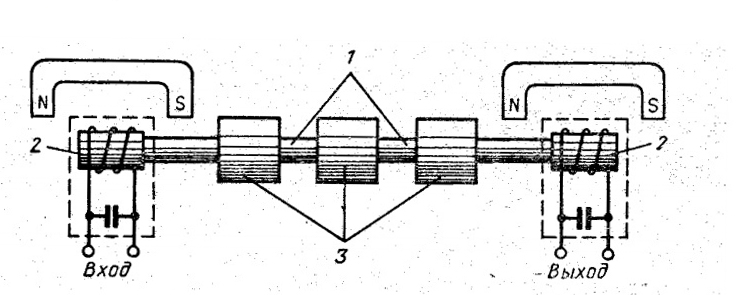
\includegraphics[width=0.8\linewidth]{fig/fig10}
	\caption{Электромеханический полосовой фильтр:
1 — связки; 2 — магнитострикционный преобразователь; 3 — резонаторы.}
	\label{fig:fig10}
\end{figure}

В зависимости от размеров каждая пластинка-резонатор имеет вполне определенную резонансную частоту, при которой наблюдаются интенсивные механические колебания. Эти колебания через металлические стерженьки-связки передаются соседнему резонатору и, если его собственная частота близка к частоте первого резонатора, возбуждают в нем также интенсивные колебания. При соответствующем подборе отдельных резонаторов и элементов связи между ними такая система обладает свойствами полосового фильтра: она пропускает без существенного затухания механические колебания только в
определенной полосе частот и создает весьма большое затухание вне этой полосы. Однако данная система связанных резонаторов является фильтром механических колебаний, поэтому для использования ее в электрических устройствах формирования однополосного сигнала на входе и выходе фильтра устанавливаются магнитострикционные преобразователи, которые преобразуют электрические колебания в механические на входе фильтра и механические колебания в электрические на выходе последнего.

В основе действия подобного типа преобразователей лежит магнитострикционный эффект, заключающийся в изменении формы и размеров ферромагнитных тел под влиянием магнитного поля. Магнитострикционный преобразователь обычно выполняется в виде катушки, в которую помещается ферромагнитный элемент, связанный с системой механических резонаторов. Для усиления эффекта магнитострикции преобразователь располагается в поле постоянного магнита, обеспечивающего постоянное подмагничивание.

Электромеханические фильтры, изготавливаемые на частоты 50 — 500 кГц, позволяют получить крутизну спада частотной характеристики порядка 0,2— 0,3 дБ/Гц и относительную полосу более $(2 - 3) 10^{-3}$. Затухание подобных
фильтров в полосе пропускания обычно не превышает единиц децибел.

Малый вес и размеры электромеханических фильтров позволяют снизить
вес и габариты аппаратуры систем однополюсной передачи. 

К недостаткам этих фильтров можно отнести трудность их изготовления, связанную с необходимостью соблюдения высокой точности обработки элементов колебательной системы.
\section{Экспериментальная часть}

\begin{figure}[H]
	\centering
	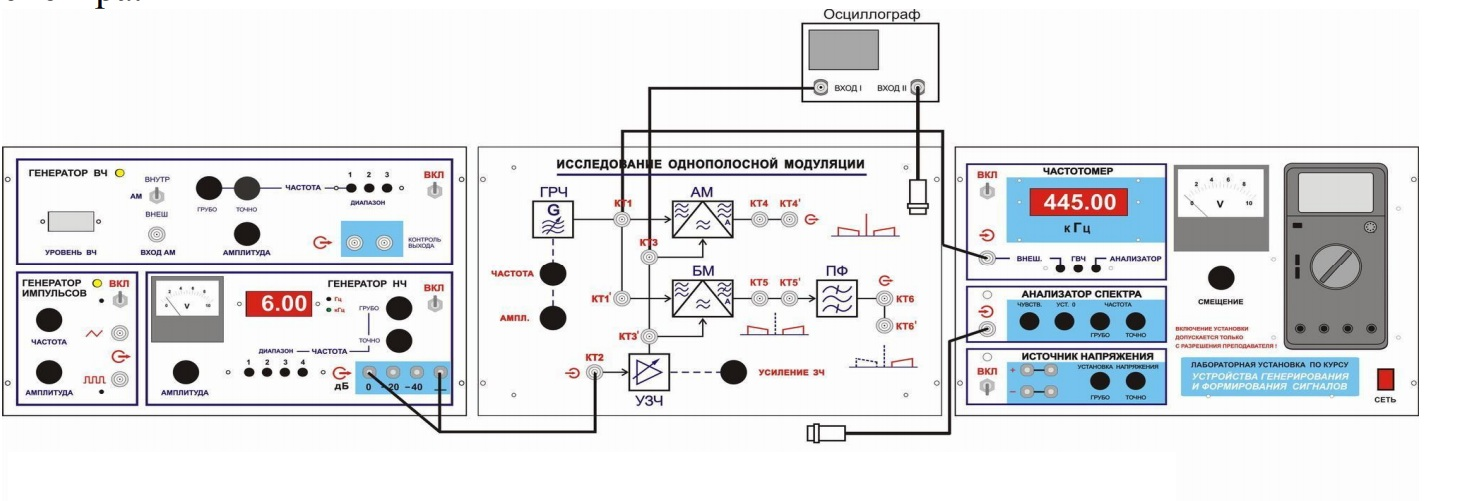
\includegraphics[width=\linewidth]{img/img00}
	\caption{Внешний вид макета}
\end{figure}


\subsection{Ознакомление с работой модулятора и параметрами АМ сигнала}

Была установлена частота ВЧ-генератора $f_{\text{вч}}=440$ кГц и максимальная амплитуда напряжения.
Была установлена частота НЧ-генератора $f_{\text{нч}}=10$ кГц и  амплитуда напряжения 
$U_{\text{НЧ}} = 1 $ В.



Наблюдали на экране осциллографа форму напряжения на выходе балансного модулятора. Пронаблюдали зависимость глубины модуляции от величины выходного напряжения НЧ-генератора.
В дальнейшем $U_{\text{нч}}$ установлено на уровень 1.0 В. Изменяя величину НЧ-напряжения, установили глубину модуляции $m=0.5$. С помощью анализатора спектра проанализировали АМ сигнал и получили:

\begin{itemize}
	\item $f_{\text{верх}}=439.6$ кГц
	\item $f_{\text{ниж}}=429.6$ кГц
	\item $f_{\text{сред}}=449.6$ кГц
\end{itemize}
На рис. \ref{fig:rec2} приведена осциллограмма исследуемого АМ-сигнала.

\begin{figure}[H]
	\centering
	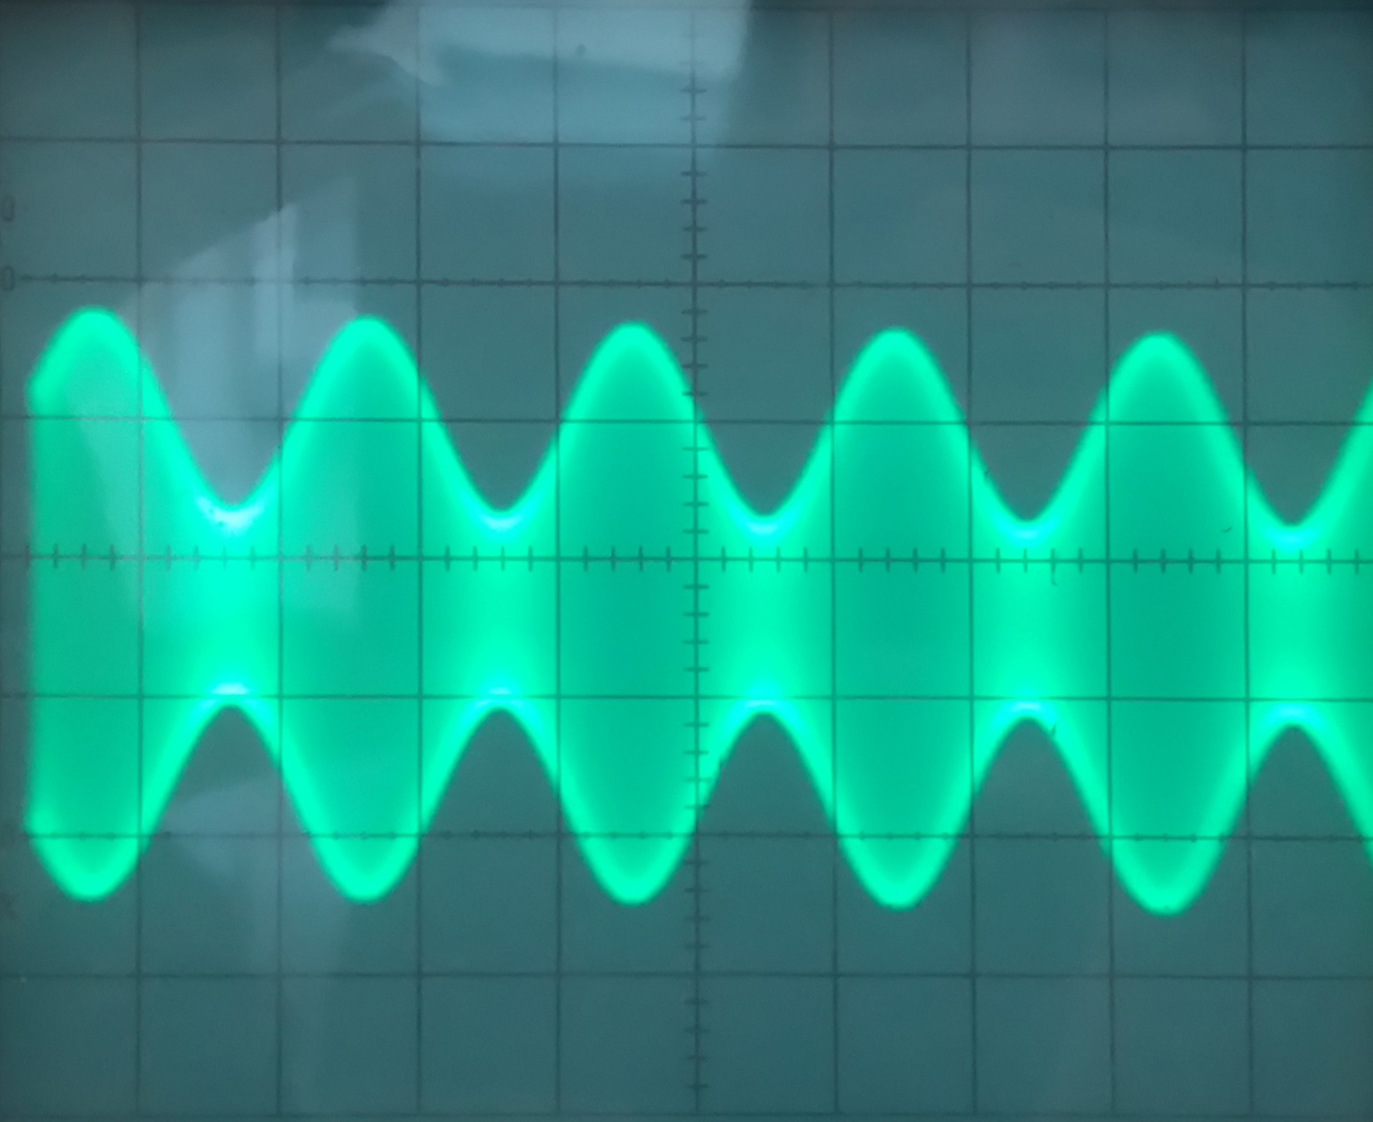
\includegraphics[width=0.7\linewidth]{img/img1}
	\caption{Осциллограмма АМ-сигнала}
	\label{fig:rec2}
\end{figure}


\subsection{Определение полосы пропускания полосового фильтра}
Выходное напряжение ВЧ-генератора установлено на уровне 0 дБ. Выходное напряжение НЧ-генератора $U_{\text{НЧ}}=0$ В.
Была снята амплитудно-частотная характеристика полосового фильтра и из рис.\ref{fig:rec1} была определена полоса пропускания ПФ и его средняя частота:

\begin{itemize}
	\item $f_{\text{верх}}=462$ кГц
	\item $f_{\text{ниж}}=448$ кГц
	\item $f_{\text{сред}}=455$ кГц
\end{itemize}

\begin{figure}[H]
	\centering
	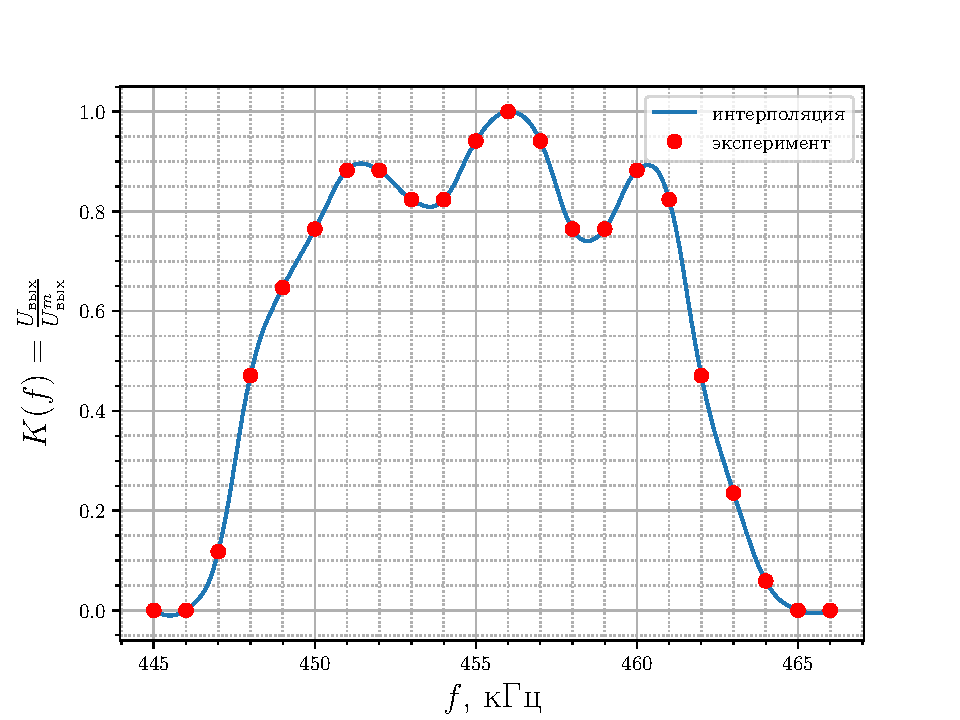
\includegraphics[width=0.7\linewidth]{fig/task1}
	\caption{Амплитудно-частотная характеристика ПФ}
	\label{fig:rec1}
\end{figure}


\subsection{Ознакомление с работой балансного амплитудного модулятора и параметрами АМ сигнала с полностью подавленной несущей}

Вход анализатора спектра соединен с гнездом $\text{КТ}5'$. Вход II осциллографа соединен с гнездом $\text{КТ}5$.

Наблюдали на экране осциллографа форму напряжения на выходе
балансного модулятора. Изменяя в некоторых пределах величину выходного
% напряжения НЧ-генератора, наблюдали изменение глубины модуляции.
% Установить UНЧ0,5. 
Определили спектральный состав сигнала:
\begin{itemize}
	\item $f_{\text{верх}}=449.6 \text{ кГц}, ~ U= 3 \text{ у.е.} $
	\item $f_{\text{ниж}}=429.6 \text{ кГц}, ~ U= 3 \text{ у.е.} $
\end{itemize}



\subsection{Ознакомление с работой однополосного модулятора и параметрами ОМ сигнала J3E}
Вход анализатора спектра соединен с гнездом $\text{КТ}6'$. Вход II осциллографа соединен с гнездом $\text{КТ}6$.
Определили спектральный состав сигнала:
\begin{itemize}
	\item $f_{\text{верх}}=449.6$ кГц, $U=6.5$ у.е.
\end{itemize}

\begin{figure}[H]
\begin{minipage}[h]{0.49\linewidth}
	\centering
	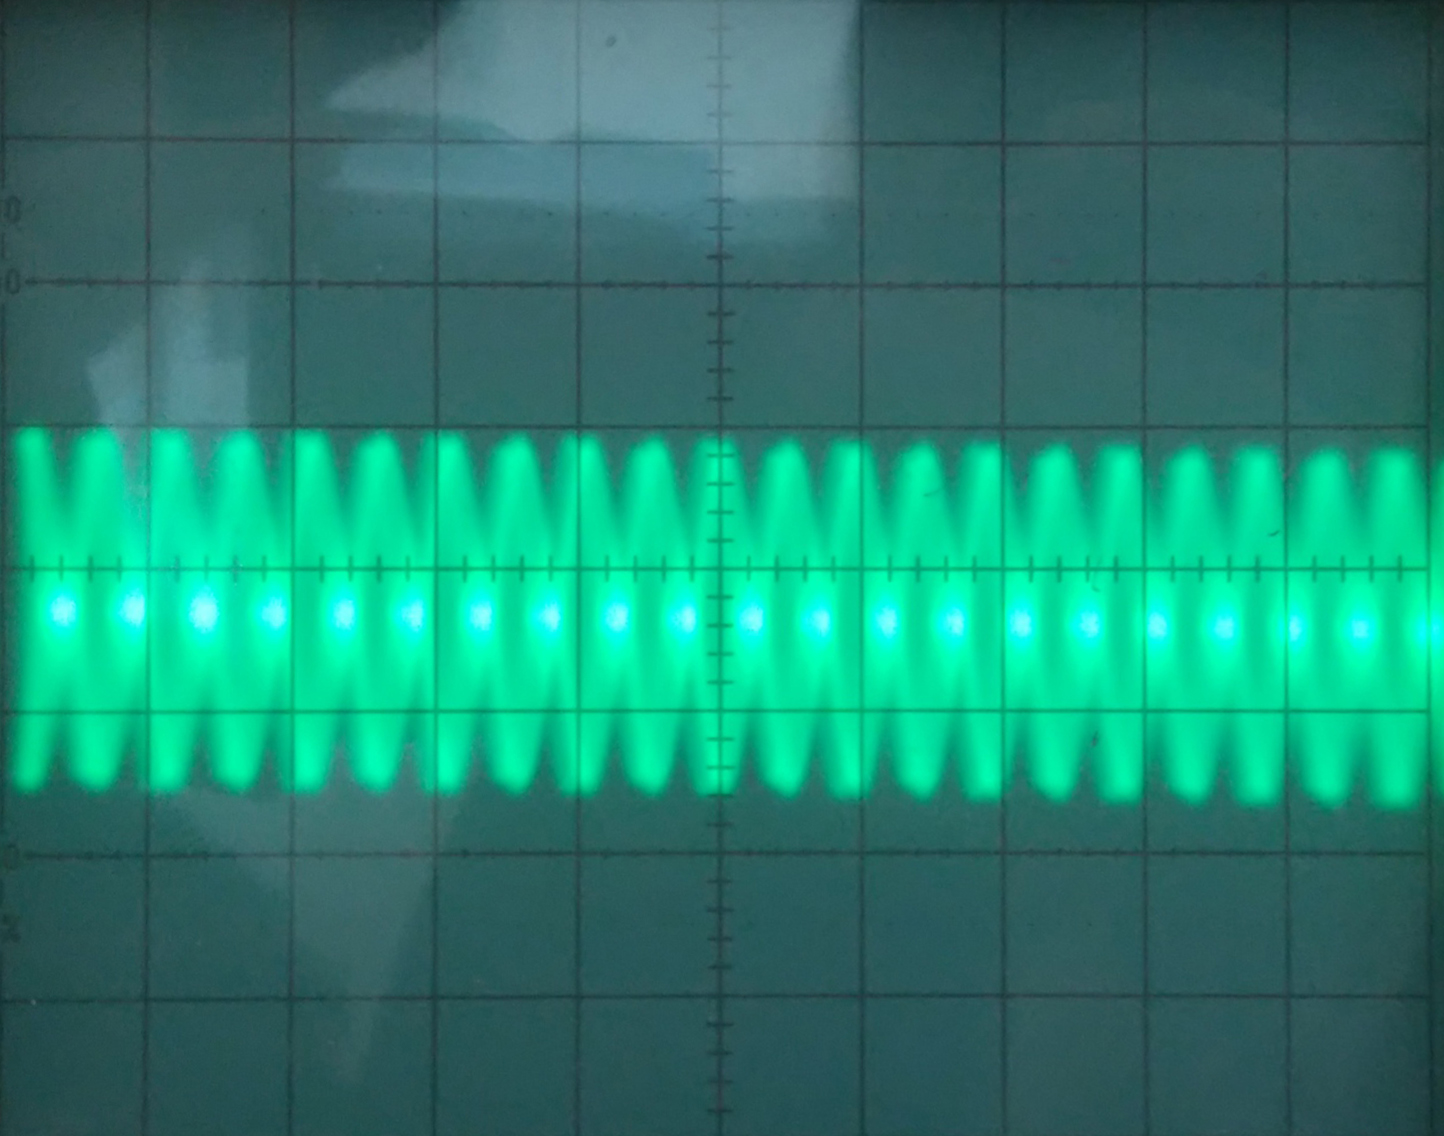
\includegraphics[width=\linewidth]{img/img4}
	\caption{Осциллограмма АМ-сигнала с полностью подавленной несущей.}
	\label{fig:rec3}
\end{minipage}
\hfill
\begin{minipage}[h]{0.49\linewidth}
	\centering
	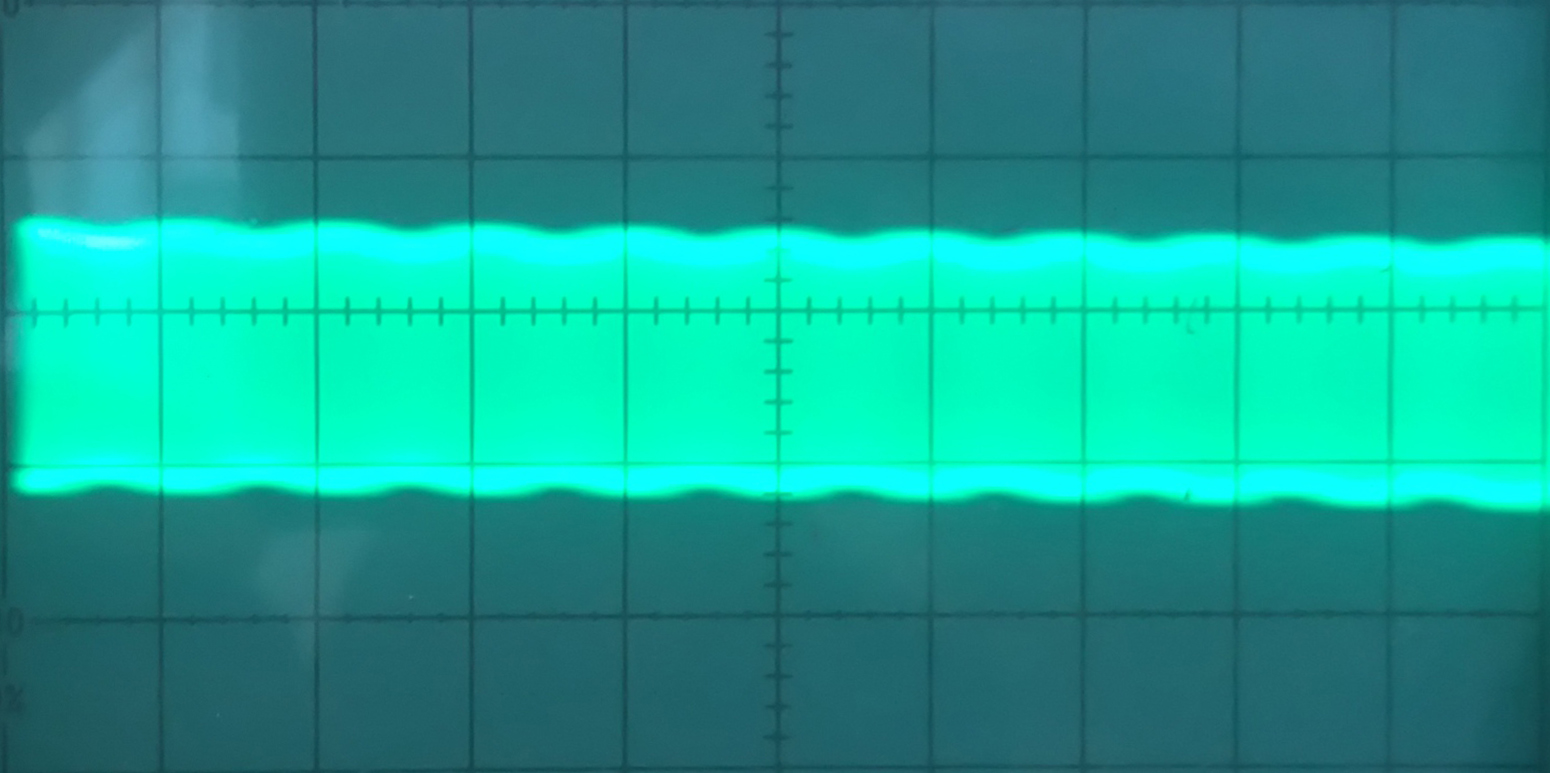
\includegraphics[width=\linewidth]{img/img3}
	\caption{Ознакомление с работой однополосного модулятора }
	\label{fig:rec4}
\end{minipage}
\end{figure}




\subsection{Определение влияния частоты модулирующего напряжения на спектральный состав АМ-сигнала}

Вход анализатора соединили с $\text{КТ4'}$, осциллограф с $\text{КТ4}$. Частоту НЧ-генератора установили $f_{\text{НЧ}}=15 \text{ кГц.}$

Спектральный состав:
\begin{itemize}
	\item $f_{\text{ниж}}=425 \text{ кГц},~ U=1 \text{ у.е.}$
	\item $f_{\text{нес}}=440 \text{ кГц},~ U=8 \text{ у.е.}$
	\item $f_{\text{верх}}=455 \text{ кГц},~ U=1 \text{ у.е.}$
\end{itemize}

После соединили анализатор с $\text{КТ5'}$, а осциллограф с $\text{КТ5}$.

Спектральный состав:
\begin{itemize}
	\item $f_{\text{верх}}=455 \text{ кГц}, ~U_{\text{верх}}=6.5 \text{ у.е.}$
\end{itemize}

Как видно из полученных данных при изменении частоты НЧ-генератора изменились частоты $f_{\text{верх}}$ и $f_{\text{ниж}}$, при этом амплитуды сохранили значения полученные ранее.
\subsection{Заключение}

В ходе данной работы мы ознакомились с основами теории работы однополосного модулятора  и проверили теоретические рассуждения на практике, наблюдали осциллограммы АМ-сигнала, АМ-сигнала с подавленной несущей и сигнала на выходе с однополосного модулятора. Все практические данные полностью соответствуют теоретическим представлениям. 
\end{document}

